%%%%%%%%%%%%%%%%%%%%%%%%%%%%%%%%%%%%%%%%%
% baposter Landscape Poster
% LaTeX Template
% Version 1.0 (11/06/13)
%
% baposter Class Created by:
% Brian Amberg (baposter@brian-amberg.de)
%
% This template has been downloaded from:
% http://www.LaTeXTemplates.com
%
% License:
% CC BY-NC-SA 3.0 (http://creativecommons.org/licenses/by-nc-sa/3.0/)
%
%%%%%%%%%%%%%%%%%%%%%%%%%%%%%%%%%%%%%%%%%

%----------------------------------------------------------------------------------------
%	PACKAGES AND OTHER DOCUMENT CONFIGURATIONS
%----------------------------------------------------------------------------------------

\documentclass[landscape,a0paper,fontscale=0.35]{baposter} % Adjust the font scale/size here : fontscale=0.285
%\usepackage{textpos}
\usepackage[frenchb]{babel}
\usepackage[T1]{fontenc}
\usepackage[utf8]{inputenc}
\usepackage{tikz}
\usepackage{graphicx} % Required for including images
%\graphicspath{{Figures/}} % Directory in which figures are stored
\usepackage{amsmath} % For typesetting math
\usepackage{amsthm}
\usepackage{amssymb} % Adds new symbols to be used in math mode
\usepackage{booktabs} % Top and bottom rules for tables
\usepackage{enumitem} % Used to reduce itemize/enumerate spacing
\usepackage{palatino} % Use the Palatino font
\usepackage[font=small,labelfont=bf]{caption} % Required for specifying captions to tables and figures
\usepackage{multicol} % Required for multiple columns
\usepackage{tikz} % Required for flow chart
\usetikzlibrary{shapes,arrows} % Tikz libraries required for the flow chart in the template
%\usepackage{dsfont}
%\usepackage{listings}
\usepackage{subfigure}
\usepackage{color}
%\usepackage{nth}
%\usepackage{a4wide}
\usepackage{graphicx,color}
\usepackage{array}
%\usepackage[nottoc, notlof, notlot]{tocbibind}
\usepackage{subfigure}
\usetikzlibrary{arrows,shapes,positioning,calc}
%\definecolor{CPU}{RGB}{30, 167, 223}
%\definecolor{CPU}{RGB}{8, 138, 104}
\definecolor{gris}{gray}{0.9}
\usepackage{geometry}
\geometry{left=0.9cm,right=0.9cm,bottom=0.9cm,top=0.9cm,centering}
%\usepackage{subfig}
\usepackage{float}
\usepackage{multicol}
\usepackage{enumitem,rotating}
\usepackage{bbm}
\usepackage{tcolorbox}


\newcommand{\sidecap}[1]{ {\begin{sideways}\parbox{0.2\textwidth}{\centering #1}\end{sideways}} }

\theoremstyle{plain}
\newtheorem*{thm}{Theorem}
%\theoremstyle{definition}
%\newtheorem*{defi}[thm]{Definition}
\theoremstyle{plain}
\newtheorem*{prop}{Properties}
\theoremstyle{plain}
\newtheorem*{hyp}{Assumption}
\theoremstyle{plain}
\newtheorem*{proposition}{Proposition}

\setlength{\columnsep}{1.5em} % Slightly increase the space between columns
\setlength{\columnseprule}{0mm} % No horizontal rule between columns

\definecolor{lightred}{rgb}{0.5 0 0}

\newcommand{\compresslist}{ % Define a command to reduce spacing within itemize/enumerate environments, this is used right after \begin{itemize} or \begin{enumerate}
\setlength{\itemsep}{1pt}
\setlength{\parskip}{0pt}
\setlength{\parsep}{0pt}
}

\definecolor{CPU}{RGB}{0, 153, 125} % Defines the color used for content box headers




% Math operators
\newcommand{\scal}[2]{\left\langle #1 , #2 \right\rangle}
\DeclareMathOperator{\IR}{\mathbb{R}}
\DeclareMathOperator*{\argmin}{argmin}
\DeclareMathOperator{\One}{\mathbbm{1}}
\DeclareMathOperator{\Ccal}{\mathcal{C}}
\DeclareMathOperator{\logsumexp}{logsumexp}
\DeclareMathOperator{\diag}{diag}
\DeclareMathOperator{\KL}{KL}
\newcommand{\norm}[1]{\left\lVert #1 \right\rVert}
\renewcommand{\epsilon}{\varepsilon}


\begin{document}

\begin{poster}
{
background=plain,
headershade=plain,
headerborder=closed, % Adds a border around the header of content boxes
colspacing=0.8em, % Column spacing
bgColorOne=gris, % Background color for the gradient on the left side of the poster
bgColorTwo=gris, % Background color for the gradient on the right side of the poster
borderColor=CPU, % Border color
headerColorOne=CPU, % Background color for the header in the content boxes (left side)
headerColorTwo=CPU, % Background color for the header in the content boxes (right side)
headerFontColor=white, % Text color for the header text in the content boxes
boxColorOne=white, % Background color of the content boxes
textborder=roundedsmall, % Format of the border around content boxes, can be: none, bars, coils, triangles, rectangle, rounded, roundedsmall, roundedright or faded
eyecatcher=true, % Set to false for ignoring the left logo in the title and move the title left
headerheight=0.10\textheight, % Height of the header
headershape=rounded, % Specify the rounded corner in the content box headers, can be: rectangle, small-rounded, roundedright, roundedleft or rounded
headerfont=\Large\bf\textsc, % Large, bold and sans serif font in the headers of content boxes
%textfont={\setlength{\parindent}{1.5em}}, % Uncomment for paragraph indentation
linewidth=1.8pt, % Width of the border lines around content boxes
columns=3,
}
%----------------------------------------------------------------------------------------
%	TITLE SECTION 
%----------------------------------------------------------------------------------------
%
{
\includegraphics[height=6em]{logo_ens_psl.png}} % First university/lab logo on the left
{\bf Overrelaxed Sinkhorn--Knopp algorithm\\ for regularized optimal transport\vspace{0.2em}} 
{{Alexis Thibault, L\'enaïc Chizat, Charles Dossal and  Nicolas Papadakis}} % Author names and institution
{
\includegraphics[height=6em]{logo_imb.png}} % Second university/lab logo on the right

%----------------------------------------------------------------------------------------
%	RESEARCH
%----------------------------------------------------------------------------------------

% Introduction

\headerbox{Introduction}{name=intro,column=0,span=2}{
	\begin{minipage}{0.55\textwidth}
		Optimal Transport is an efficient and flexible tool to compare two probability distributions. It has been popularized in the computer vision community in the context of discrete histograms. The introduction of entropic regularization in [Cuturi, 2013] has made possible the use of the fast Sinkhorn--Knopp algorithm (SK) [Sinkhorn, 1964] scaling with high dimensional data.
		
		For small regularization $\epsilon$, the SK algorithm becomes extremely slow. To counter this, we propose a new algorithm that accelerates SK by \emph{overrelaxation}.
		This idea has been shown to successfully accelerate the algorithm. However, there is no proof of convergence in the literature, and no automated choice of parameters.
		In our paper, we suggest a way of ensuring global convergence. This is done simply by choosing the overrelaxation parameters at each step of the algorithm so that a given function decreases. We will motivate our choice of function with numerical results.
		
		The algorithm we obtain converges faster than Sinkhorn--Knopp, while remaining parallelizable, and having almost the same cost per iteration.
	\end{minipage}
	\begin{minipage}{0.45\textwidth}
		\centering
		\begin{tcolorbox}[width=0.99\textwidth,/tcb/size=small, /tcb/top=2.0mm]
			\centering
			\begin{tabular}{c c c c}
				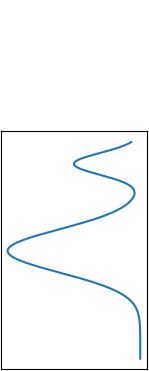
\includegraphics[height=3cm]{1d_interp_mu} &
				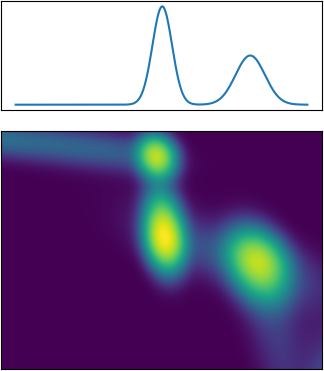
\includegraphics[height=3cm]{1d_interp_0_2} &
				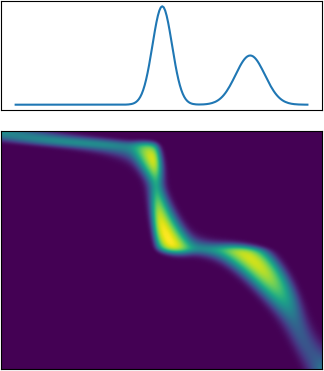
\includegraphics[height=3cm]{1d_interp_2} &
				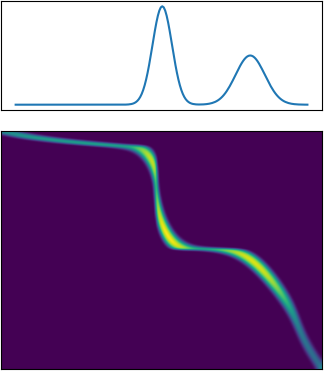
\includegraphics[height=3cm]{1d_interp_18} \\
				&
				$\epsilon = 5$ &
				$\epsilon = 0.5$ &
				$\epsilon = 0.02$
			\end{tabular}
			\captionof{figure}{Regularized optimal transport maps for decreasing regularization parameter $\epsilon$.} \label{fig:1d_ot}
		\end{tcolorbox}
	\end{minipage}
}




%----------------------------------------------------------------------------------------
%	
%----------------------------------------------------------------------------------------

\headerbox{Overrelaxation}{name=overrelaxation,column=2}{
\begin{minipage}{0.49\textwidth}
	\begin{tcolorbox}[size=small, top=2mm]
		\centering
		\begin{tabular}{c c}
		\begin{tikzpicture}
\fill (-0.500000,4.000000) circle (2pt) node[above] (gamma0) {$\gamma^0$};
\fill (0,0) circle (2pt) node[right] {$\gamma^*$};
\draw[dashed] (-0.500000,4.000000) -- (0.000000,4.000000)
(-0.995851,3.734440) -- (0.000000,4.000000)
(-0.995851,3.734440) -- (0.000000,3.734440)
(-0.929736,3.486510) -- (0.000000,3.734440)
(-0.929736,3.486510) -- (0.000000,3.486510)
(-0.868011,3.255041) -- (0.000000,3.486510)
(-0.868011,3.255041) -- (0.000000,3.255041)
(-0.810384,3.038938) -- (0.000000,3.255041)
(-0.810384,3.038938) -- (0.000000,3.038938)
(-0.756582,2.837183) -- (0.000000,3.038938)
(-0.756582,2.837183) -- (0.000000,2.837183)
(-0.706353,2.648822) -- (0.000000,2.837183)
(-0.706353,2.648822) -- (0.000000,2.648822)
(-0.659458,2.472967) -- (0.000000,2.648822)
(-0.659458,2.472967) -- (0.000000,2.472967)
(-0.615676,2.308787) -- (0.000000,2.472967)
(-0.615676,2.308787) -- (0.000000,2.308787)
(-0.574802,2.155506) -- (0.000000,2.308787)
(-0.574802,2.155506) -- (0.000000,2.155506)
(-0.536641,2.012402) -- (0.000000,2.155506)
(-0.536641,2.012402) -- (0.000000,2.012402)
(-0.501013,1.878799) -- (0.000000,2.012402)
(-0.501013,1.878799) -- (0.000000,1.878799)
(-0.467751,1.754065) -- (0.000000,1.878799)
(-0.467751,1.754065) -- (0.000000,1.754065)
(-0.436697,1.637613) -- (0.000000,1.754065)
(-0.436697,1.637613) -- (0.000000,1.637613)
(-0.407704,1.528891) -- (0.000000,1.637613)
(-0.407704,1.528891) -- (0.000000,1.528891)
(-0.380637,1.427388) -- (0.000000,1.528891)
(-0.380637,1.427388) -- (0.000000,1.427388)
(-0.355366,1.332624) -- (0.000000,1.427388)
(-0.355366,1.332624) -- (0.000000,1.332624)
(-0.331774,1.244151) -- (0.000000,1.332624)
(-0.331774,1.244151) -- (0.000000,1.244151)
(-0.309747,1.161552) -- (0.000000,1.244151)
(-0.309747,1.161552) -- (0.000000,1.161552)
(-0.289183,1.084436) -- (0.000000,1.161552)
(-0.289183,1.084436) -- (0.000000,1.084436)
(-0.269984,1.012440) -- (0.000000,1.084436)
(-0.269984,1.012440) -- (0.000000,1.012440)
(-0.252060,0.945225) -- (0.000000,1.012440)
(-0.252060,0.945225) -- (0.000000,0.945225)
(-0.235326,0.882471) -- (0.000000,0.945225)
(-0.235326,0.882471) -- (0.000000,0.882471)
(-0.219702,0.823884) -- (0.000000,0.882471)
(-0.219702,0.823884) -- (0.000000,0.823884)
(-0.205116,0.769186) -- (0.000000,0.823884)
(-0.205116,0.769186) -- (0.000000,0.769186)
(-0.191499,0.718120) -- (0.000000,0.769186)
(-0.191499,0.718120) -- (0.000000,0.718120)
(-0.178785,0.670444) -- (0.000000,0.718120)
(-0.178785,0.670444) -- (0.000000,0.670444)
(-0.166915,0.625933) -- (0.000000,0.670444)
(-0.166915,0.625933) -- (0.000000,0.625933)
(-0.155834,0.584377) -- (0.000000,0.625933)
(-0.155834,0.584377) -- (0.000000,0.584377)
(-0.145488,0.545580) -- (0.000000,0.584377)
(-0.145488,0.545580) -- (0.000000,0.545580)
(-0.135829,0.509359) -- (0.000000,0.545580)
(-0.135829,0.509359) -- (0.000000,0.509359)
(-0.126811,0.475543) -- (0.000000,0.509359)
(-0.126811,0.475543) -- (0.000000,0.475543)
(-0.118392,0.443972) -- (0.000000,0.475543)
(-0.118392,0.443972) -- (0.000000,0.443972)
(-0.110532,0.414496) -- (0.000000,0.443972)
(-0.110532,0.414496) -- (0.000000,0.414496)
(-0.103194,0.386978) -- (0.000000,0.414496)
(-0.103194,0.386978) -- (0.000000,0.386978)
(-0.096343,0.361286) -- (0.000000,0.386978)
(-0.096343,0.361286) -- (0.000000,0.361286)
(-0.089947,0.337301) -- (0.000000,0.361286)
(-0.089947,0.337301) -- (0.000000,0.337301)
(-0.083975,0.314907) -- (0.000000,0.337301)
(-0.083975,0.314907) -- (0.000000,0.314907)
(-0.078400,0.294000) -- (0.000000,0.314907)
(-0.078400,0.294000) -- (0.000000,0.294000)
(-0.073195,0.274482) -- (0.000000,0.294000)
(-0.073195,0.274482) -- (0.000000,0.274482)
(-0.068336,0.256259) -- (0.000000,0.274482)
(-0.068336,0.256259) -- (0.000000,0.256259)
(-0.063799,0.239246) -- (0.000000,0.256259)
(-0.063799,0.239246) -- (0.000000,0.239246)
(-0.059563,0.223362) -- (0.000000,0.239246)
(-0.059563,0.223362) -- (0.000000,0.223362)
(-0.055609,0.208533) -- (0.000000,0.223362)
(-0.055609,0.208533) -- (0.000000,0.208533)
(-0.051917,0.194689) -- (0.000000,0.208533)
(-0.051917,0.194689) -- (0.000000,0.194689)
(-0.048470,0.181763) -- (0.000000,0.194689)
(-0.048470,0.181763) -- (0.000000,0.181763)
(-0.045252,0.169696) -- (0.000000,0.181763)
(-0.045252,0.169696) -- (0.000000,0.169696)
(-0.042248,0.158430) -- (0.000000,0.169696)
(-0.042248,0.158430) -- (0.000000,0.158430)
(-0.039443,0.147912) -- (0.000000,0.158430)
(-0.039443,0.147912) -- (0.000000,0.147912)
(-0.036825,0.138092) -- (0.000000,0.147912)
(-0.036825,0.138092) -- (0.000000,0.138092)
(-0.034380,0.128924) -- (0.000000,0.138092)
(-0.034380,0.128924) -- (0.000000,0.128924)
(-0.032097,0.120365) -- (0.000000,0.128924)
(-0.032097,0.120365) -- (0.000000,0.120365)
(-0.029966,0.112374) -- (0.000000,0.120365)
(-0.029966,0.112374) -- (0.000000,0.112374)
(-0.027977,0.104913) -- (0.000000,0.112374)
(-0.027977,0.104913) -- (0.000000,0.104913)
(-0.026119,0.097948) -- (0.000000,0.104913)
(-0.026119,0.097948) -- (0.000000,0.097948)
(-0.024385,0.091445) -- (0.000000,0.097948)
(-0.024385,0.091445) -- (0.000000,0.091445)
(-0.022766,0.085374) -- (0.000000,0.091445)
(-0.022766,0.085374) -- (0.000000,0.085374)
(-0.021255,0.079706) -- (0.000000,0.085374)
(-0.021255,0.079706) -- (0.000000,0.079706)
(-0.019844,0.074415) -- (0.000000,0.079706)
(-0.019844,0.074415) -- (0.000000,0.074415)
(-0.018526,0.069474) -- (0.000000,0.074415)
(-0.018526,0.069474) -- (0.000000,0.069474)
(-0.017296,0.064862) -- (0.000000,0.069474)
(-0.017296,0.064862) -- (0.000000,0.064862)
(-0.016148,0.060556) -- (0.000000,0.064862)
(-0.016148,0.060556) -- (0.000000,0.060556)
(-0.015076,0.056535) -- (0.000000,0.060556)
(-0.015076,0.056535) -- (0.000000,0.056535)
(-0.014075,0.052782) -- (0.000000,0.056535)
(-0.014075,0.052782) -- (0.000000,0.052782)
(-0.013141,0.049278) -- (0.000000,0.052782)
(-0.013141,0.049278) -- (0.000000,0.049278)
(-0.012268,0.046006) -- (0.000000,0.049278)
(-0.012268,0.046006) -- (0.000000,0.046006)
(-0.011454,0.042952) -- (0.000000,0.046006)
(-0.011454,0.042952) -- (0.000000,0.042952)
(-0.010693,0.040100) -- (0.000000,0.042952)
(-0.010693,0.040100) -- (0.000000,0.040100)
(-0.009983,0.037438) -- (0.000000,0.040100)
(-0.009983,0.037438) -- (0.000000,0.037438)
(-0.009321,0.034952) -- (0.000000,0.037438)
(-0.009321,0.034952) -- (0.000000,0.034952)
(-0.008702,0.032632) -- (0.000000,0.034952)
(-0.008702,0.032632) -- (0.000000,0.032632)
(-0.008124,0.030466) -- (0.000000,0.032632)
(-0.008124,0.030466) -- (0.000000,0.030466)
(-0.007585,0.028443) -- (0.000000,0.030466)
(-0.007585,0.028443) -- (0.000000,0.028443)
(-0.007081,0.026555) -- (0.000000,0.028443)
(-0.007081,0.026555) -- (0.000000,0.026555)
(-0.006611,0.024792) -- (0.000000,0.026555)
(-0.006611,0.024792) -- (0.000000,0.024792)
(-0.006172,0.023146) -- (0.000000,0.024792)
(-0.006172,0.023146) -- (0.000000,0.023146)
(-0.005762,0.021609) -- (0.000000,0.023146)
(-0.005762,0.021609) -- (0.000000,0.021609)
(-0.005380,0.020174) -- (0.000000,0.021609)
(-0.005380,0.020174) -- (0.000000,0.020174)
(-0.005023,0.018835) -- (0.000000,0.020174)
(-0.005023,0.018835) -- (0.000000,0.018835)
(-0.004689,0.017585) -- (0.000000,0.018835)
(-0.004689,0.017585) -- (0.000000,0.017585)
(-0.004378,0.016417) -- (0.000000,0.017585)
(-0.004378,0.016417) -- (0.000000,0.016417)
(-0.004087,0.015327) -- (0.000000,0.016417)
(-0.004087,0.015327) -- (0.000000,0.015327)
(-0.003816,0.014310) -- (0.000000,0.015327)
(-0.003816,0.014310) -- (0.000000,0.014310)
(-0.003563,0.013360) -- (0.000000,0.014310)
(-0.003563,0.013360) -- (0.000000,0.013360)
(-0.003326,0.012473) -- (0.000000,0.013360)
(-0.003326,0.012473) -- (0.000000,0.012473)
(-0.003105,0.011645) -- (0.000000,0.012473)
(-0.003105,0.011645) -- (0.000000,0.011645)
(-0.002899,0.010872) -- (0.000000,0.011645)
(-0.002899,0.010872) -- (0.000000,0.010872)
(-0.002707,0.010150) -- (0.000000,0.010872)
(-0.002707,0.010150) -- (0.000000,0.010150)
(-0.002527,0.009476) -- (0.000000,0.010150)
(-0.002527,0.009476) -- (0.000000,0.009476)
(-0.002359,0.008847) -- (0.000000,0.009476)
(-0.002359,0.008847) -- (0.000000,0.008847)
(-0.002203,0.008259) -- (0.000000,0.008847)
(-0.002203,0.008259) -- (0.000000,0.008259)
(-0.002056,0.007711) -- (0.000000,0.008259)
(-0.002056,0.007711) -- (0.000000,0.007711)
(-0.001920,0.007199) -- (0.000000,0.007711)
(-0.001920,0.007199) -- (0.000000,0.007199)
(-0.001792,0.006721) -- (0.000000,0.007199)
(-0.001792,0.006721) -- (0.000000,0.006721)
(-0.001673,0.006275) -- (0.000000,0.006721)
(-0.001673,0.006275) -- (0.000000,0.006275)
(-0.001562,0.005858) -- (0.000000,0.006275)
(-0.001562,0.005858) -- (0.000000,0.005858)
(-0.001459,0.005469) -- (0.000000,0.005858)
(-0.001459,0.005469) -- (0.000000,0.005469)
(-0.001362,0.005106) -- (0.000000,0.005469)
(-0.001362,0.005106) -- (0.000000,0.005106)
(-0.001271,0.004767) -- (0.000000,0.005106)
(-0.001271,0.004767) -- (0.000000,0.004767)
(-0.001187,0.004451) -- (0.000000,0.004767)
(-0.001187,0.004451) -- (0.000000,0.004451)
(-0.001108,0.004155) -- (0.000000,0.004451)
;
\draw (-0.000000,-0.400000) -- (0.000000,4.400000) node[right] {$\mathcal{C}_1$};
\draw (0.106667,-0.400000) -- (-1.173333,4.400000) node[right] {$\mathcal{C}_2$};
\end{tikzpicture}
 &
		\begin{tikzpicture}
\fill (-0.500000,4.000000) circle (2pt) node[above] (gamma0) {$\gamma^0$};
\fill (0,0) circle (2pt) node[right] {$\gamma^*$};
\draw[dashed] (-0.500000,4.000000) -- (0.350000,4.000000)
(-1.898444,3.400415) -- (0.350000,4.000000)
(-1.898444,3.400415) -- (1.328911,3.400415)
(-2.219432,2.454190) -- (1.328911,3.400415)
(-2.219432,2.454190) -- (1.553603,2.454190)
(-1.950880,1.519661) -- (1.553603,2.454190)
(-1.950880,1.519661) -- (1.365616,1.519661)
(-1.444980,0.770169) -- (1.365616,1.519661)
(-1.444980,0.770169) -- (1.011486,0.770169)
(-0.919844,0.255148) -- (1.011486,0.770169)
(-0.919844,0.255148) -- (0.643891,0.255148)
(-0.486040,-0.046167) -- (0.643891,0.255148)
(-0.486040,-0.046167) -- (0.340228,-0.046167)
(-0.180221,-0.184954) -- (0.340228,-0.046167)
(-0.180221,-0.184954) -- (0.126154,-0.184954)
(0.004209,-0.217472) -- (0.126154,-0.184954)
(0.004209,-0.217472) -- (-0.002946,-0.217472)
(0.093772,-0.191681) -- (-0.002946,-0.217472)
(0.093772,-0.191681) -- (-0.065641,-0.191681)
(0.119666,-0.142266) -- (-0.065641,-0.191681)
(0.119666,-0.142266) -- (-0.083766,-0.142266)
(0.109394,-0.090756) -- (-0.083766,-0.142266)
(0.109394,-0.090756) -- (-0.076576,-0.090756)
(0.083372,-0.048103) -- (-0.076576,-0.090756)
(0.083372,-0.048103) -- (-0.058360,-0.048103)
(0.054625,-0.017974) -- (-0.058360,-0.048103)
(0.054625,-0.017974) -- (-0.038237,-0.017974)
(0.030058,0.000238) -- (-0.038237,-0.017974)
(0.030058,0.000238) -- (-0.021040,0.000238)
(0.012253,0.009116) -- (-0.021040,0.000238)
(0.012253,0.009116) -- (-0.008577,0.009116)
(0.001178,0.011717) -- (-0.008577,0.009116)
(0.001178,0.011717) -- (-0.000824,0.011717)
(-0.004475,0.010744) -- (-0.000824,0.011717)
(-0.004475,0.010744) -- (0.003133,0.010744)
(-0.006387,0.008205) -- (0.003133,0.010744)
(-0.006387,0.008205) -- (0.004471,0.008205)
(-0.006098,0.005387) -- (0.004471,0.008205)
(-0.006098,0.005387) -- (0.004268,0.005387)
(-0.004786,0.002973) -- (0.004268,0.005387)
(-0.004786,0.002973) -- (0.003350,0.002973)
(-0.003225,0.001219) -- (0.003350,0.002973)
(-0.003225,0.001219) -- (0.002258,0.001219)
(-0.001842,0.000126) -- (0.002258,0.001219)
(-0.001842,0.000126) -- (0.001289,0.000126)
(-0.000810,-0.000434) -- (0.001289,0.000126)
(-0.000810,-0.000434) -- (0.000567,-0.000434)
(-0.000149,-0.000625) -- (0.000567,-0.000434)
(-0.000149,-0.000625) -- (0.000105,-0.000625)
(0.000203,-0.000599) -- (0.000105,-0.000625)
(0.000203,-0.000599) -- (-0.000142,-0.000599)
(0.000337,-0.000471) -- (-0.000142,-0.000599)
(0.000337,-0.000471) -- (-0.000236,-0.000471)
(0.000338,-0.000318) -- (-0.000236,-0.000471)
(0.000338,-0.000318) -- (-0.000236,-0.000318)
(0.000273,-0.000182) -- (-0.000236,-0.000318)
(0.000273,-0.000182) -- (-0.000191,-0.000182)
(0.000189,-0.000080) -- (-0.000191,-0.000182)
(0.000189,-0.000080) -- (-0.000133,-0.000080)
(0.000112,-0.000015) -- (-0.000133,-0.000080)
(0.000112,-0.000015) -- (-0.000078,-0.000015)
(0.000052,0.000020) -- (-0.000078,-0.000015)
(0.000052,0.000020) -- (-0.000037,0.000020)
(0.000013,0.000033) -- (-0.000037,0.000020)
(0.000013,0.000033) -- (-0.000009,0.000033)
(-0.000008,0.000033) -- (-0.000009,0.000033)
(-0.000008,0.000033) -- (0.000006,0.000033)
(-0.000018,0.000027) -- (0.000006,0.000033)
(-0.000018,0.000027) -- (0.000012,0.000027)
(-0.000019,0.000019) -- (0.000012,0.000027)
(-0.000019,0.000019) -- (0.000013,0.000019)
(-0.000016,0.000011) -- (0.000013,0.000019)
(-0.000016,0.000011) -- (0.000011,0.000011)
(-0.000011,0.000005) -- (0.000011,0.000011)
(-0.000011,0.000005) -- (0.000008,0.000005)
(-0.000007,0.000001) -- (0.000008,0.000005)
(-0.000007,0.000001) -- (0.000005,0.000001)
(-0.000003,-0.000001) -- (0.000005,0.000001)
(-0.000003,-0.000001) -- (0.000002,-0.000001)
(-0.000001,-0.000002) -- (0.000002,-0.000001)
(-0.000001,-0.000002) -- (0.000001,-0.000002)
(0.000000,-0.000002) -- (0.000001,-0.000002)
(0.000000,-0.000002) -- (-0.000000,-0.000002)
(0.000001,-0.000002) -- (-0.000000,-0.000002)
(0.000001,-0.000002) -- (-0.000001,-0.000002)
(0.000001,-0.000001) -- (-0.000001,-0.000002)
(0.000001,-0.000001) -- (-0.000001,-0.000001)
(0.000001,-0.000001) -- (-0.000001,-0.000001)
(0.000001,-0.000001) -- (-0.000001,-0.000001)
(0.000001,-0.000000) -- (-0.000001,-0.000001)
(0.000001,-0.000000) -- (-0.000000,-0.000000)
(0.000000,-0.000000) -- (-0.000000,-0.000000)
(0.000000,-0.000000) -- (-0.000000,-0.000000)
(0.000000,0.000000) -- (-0.000000,-0.000000)
(0.000000,0.000000) -- (-0.000000,0.000000)
(0.000000,0.000000) -- (-0.000000,0.000000)
(0.000000,0.000000) -- (-0.000000,0.000000)
(-0.000000,0.000000) -- (-0.000000,0.000000)
(-0.000000,0.000000) -- (0.000000,0.000000)
(-0.000000,0.000000) -- (0.000000,0.000000)
(-0.000000,0.000000) -- (0.000000,0.000000)
(-0.000000,0.000000) -- (0.000000,0.000000)
(-0.000000,0.000000) -- (0.000000,0.000000)
(-0.000000,0.000000) -- (0.000000,0.000000)
(-0.000000,0.000000) -- (0.000000,0.000000)
(-0.000000,0.000000) -- (0.000000,0.000000)
(-0.000000,0.000000) -- (0.000000,0.000000)
(-0.000000,0.000000) -- (0.000000,0.000000)
(-0.000000,0.000000) -- (0.000000,0.000000)
(-0.000000,-0.000000) -- (0.000000,0.000000)
(-0.000000,-0.000000) -- (0.000000,-0.000000)
(-0.000000,-0.000000) -- (0.000000,-0.000000)
(-0.000000,-0.000000) -- (0.000000,-0.000000)
(-0.000000,-0.000000) -- (0.000000,-0.000000)
(-0.000000,-0.000000) -- (0.000000,-0.000000)
(0.000000,-0.000000) -- (0.000000,-0.000000)
(0.000000,-0.000000) -- (-0.000000,-0.000000)
(0.000000,-0.000000) -- (-0.000000,-0.000000)
(0.000000,-0.000000) -- (-0.000000,-0.000000)
(0.000000,-0.000000) -- (-0.000000,-0.000000)
(0.000000,-0.000000) -- (-0.000000,-0.000000)
(0.000000,-0.000000) -- (-0.000000,-0.000000)
(0.000000,-0.000000) -- (-0.000000,-0.000000)
(0.000000,-0.000000) -- (-0.000000,-0.000000)
(0.000000,-0.000000) -- (-0.000000,-0.000000)
(0.000000,-0.000000) -- (-0.000000,-0.000000)
(0.000000,-0.000000) -- (-0.000000,-0.000000)
(0.000000,0.000000) -- (-0.000000,-0.000000)
(0.000000,0.000000) -- (-0.000000,0.000000)
(0.000000,0.000000) -- (-0.000000,0.000000)
(0.000000,0.000000) -- (-0.000000,0.000000)
(-0.000000,0.000000) -- (-0.000000,0.000000)
(-0.000000,0.000000) -- (0.000000,0.000000)
(-0.000000,0.000000) -- (0.000000,0.000000)
(-0.000000,0.000000) -- (0.000000,0.000000)
(-0.000000,0.000000) -- (0.000000,0.000000)
(-0.000000,0.000000) -- (0.000000,0.000000)
(-0.000000,0.000000) -- (0.000000,0.000000)
(-0.000000,0.000000) -- (0.000000,0.000000)
(-0.000000,0.000000) -- (0.000000,0.000000)
(-0.000000,0.000000) -- (0.000000,0.000000)
(-0.000000,0.000000) -- (0.000000,0.000000)
(-0.000000,0.000000) -- (0.000000,0.000000)
(-0.000000,-0.000000) -- (0.000000,0.000000)
(-0.000000,-0.000000) -- (0.000000,-0.000000)
(-0.000000,-0.000000) -- (0.000000,-0.000000)
(-0.000000,-0.000000) -- (0.000000,-0.000000)
(0.000000,-0.000000) -- (0.000000,-0.000000)
(0.000000,-0.000000) -- (-0.000000,-0.000000)
(0.000000,-0.000000) -- (-0.000000,-0.000000)
(0.000000,-0.000000) -- (-0.000000,-0.000000)
(0.000000,-0.000000) -- (-0.000000,-0.000000)
(0.000000,-0.000000) -- (-0.000000,-0.000000)
(0.000000,-0.000000) -- (-0.000000,-0.000000)
(0.000000,-0.000000) -- (-0.000000,-0.000000)
(0.000000,-0.000000) -- (-0.000000,-0.000000)
(0.000000,-0.000000) -- (-0.000000,-0.000000)
(0.000000,-0.000000) -- (-0.000000,-0.000000)
(0.000000,-0.000000) -- (-0.000000,-0.000000)
(0.000000,0.000000) -- (-0.000000,-0.000000)
(0.000000,0.000000) -- (-0.000000,0.000000)
(0.000000,0.000000) -- (-0.000000,0.000000)
(0.000000,0.000000) -- (-0.000000,0.000000)
(-0.000000,0.000000) -- (-0.000000,0.000000)
(-0.000000,0.000000) -- (0.000000,0.000000)
(-0.000000,0.000000) -- (0.000000,0.000000)
(-0.000000,0.000000) -- (0.000000,0.000000)
(-0.000000,0.000000) -- (0.000000,0.000000)
(-0.000000,0.000000) -- (0.000000,0.000000)
(-0.000000,0.000000) -- (0.000000,0.000000)
(-0.000000,0.000000) -- (0.000000,0.000000)
(-0.000000,0.000000) -- (0.000000,0.000000)
(-0.000000,0.000000) -- (0.000000,0.000000)
(-0.000000,0.000000) -- (0.000000,0.000000)
(-0.000000,0.000000) -- (0.000000,0.000000)
(-0.000000,-0.000000) -- (0.000000,0.000000)
(-0.000000,-0.000000) -- (0.000000,-0.000000)
(-0.000000,-0.000000) -- (0.000000,-0.000000)
(-0.000000,-0.000000) -- (0.000000,-0.000000)
(0.000000,-0.000000) -- (0.000000,-0.000000)
(0.000000,-0.000000) -- (-0.000000,-0.000000)
(0.000000,-0.000000) -- (-0.000000,-0.000000)
(0.000000,-0.000000) -- (-0.000000,-0.000000)
(0.000000,-0.000000) -- (-0.000000,-0.000000)
(0.000000,-0.000000) -- (-0.000000,-0.000000)
(0.000000,-0.000000) -- (-0.000000,-0.000000)
(0.000000,-0.000000) -- (-0.000000,-0.000000)
(0.000000,-0.000000) -- (-0.000000,-0.000000)
(0.000000,-0.000000) -- (-0.000000,-0.000000)
(0.000000,-0.000000) -- (-0.000000,-0.000000)
(0.000000,-0.000000) -- (-0.000000,-0.000000)
(0.000000,0.000000) -- (-0.000000,-0.000000)
(0.000000,0.000000) -- (-0.000000,0.000000)
(0.000000,0.000000) -- (-0.000000,0.000000)
(0.000000,0.000000) -- (-0.000000,0.000000)
(0.000000,0.000000) -- (-0.000000,0.000000)
(0.000000,0.000000) -- (-0.000000,0.000000)
(-0.000000,0.000000) -- (-0.000000,0.000000)
(-0.000000,0.000000) -- (0.000000,0.000000)
(-0.000000,0.000000) -- (0.000000,0.000000)
;
\draw (-0.000000,-0.400000) -- (0.000000,4.400000) node[right] {$\mathcal{C}_1$};
\draw (0.106667,-0.400000) -- (-1.173333,4.400000) node[right] {$\mathcal{C}_2$};
\end{tikzpicture}
 \\
		SK &
		Overrelaxed SK
		\end{tabular}
	\captionof{figure}{For small regularization $\epsilon$, the SK algorithm converges slowly, whereas the overrelaxed SK algorithm converges with a better rate}
	\end{tcolorbox}
\end{minipage}
\begin{minipage}{0.49\textwidth}
	\vspace{0.6mm}
	Although the SK algorithm is much more efficient than linear solvers in a high-dimensional setting, it becomes extremely slow when the regularization $\epsilon$ is small.
	To counteract this limitation, we use the principle of \emph{overrelaxation}.
	
	We define the overrelaxed projections of parameter $\theta \in \IR$:
	\begin{align*}\label{or_scaling}
	P_{\Ccal_1}^\theta(\gamma) &= \diag(a)^\theta \gamma\\
	P_{\Ccal_2}^\theta(\gamma) &= \gamma \diag(b)^\theta \nonumber .
	\end{align*}
	In these equations, the exponentiation is applied element-wise.
	
	In the euclidean setting, which also corresponds to the linearization of the operators around the solution, iterative overrelaxed projections can be shown to converge for any $\theta \in (0,2)$.
\end{minipage}
}

%----------------------------------------------------------------------------------------
%	Bootstrap
%----------------------------------------------------------------------------------------

\headerbox{Experiments}{name=expe,below=overrelaxation,column=2}{
	\begin{minipage}{\textwidth}
		We compare our algorithm to SK algorithm on two different optimal transport settings.
		\begin{itemize}
			\item In setting (a) we consider the domain $[0,1]$ discretized into $100$ samples and the squared Euclidean transport cost on this domain.
			The marginals are densities made of the sum of a base plateau of height $0.1$ and another plateau of height and boundaries chosen uniformly in $[0,1]$, subsequently normalized.
			\item In setting (b) the cost is a $100\times 100$ random matrix with entries uniform in $[0,1]$ and the marginals are uniform.
		\end{itemize}
		We plot the relative speed of our algorithm compared to Sinkhorn, for various values of the regularization parameter $\epsilon$. In both experimental settings, our algorithm wins by a factor above $20$ for small values of $\epsilon$.
	\end{minipage}
	\begin{minipage}{\textwidth}
		\begin{tcolorbox}[size=small]
			\begin{minipage}[b]{.5\linewidth}
				\centering
				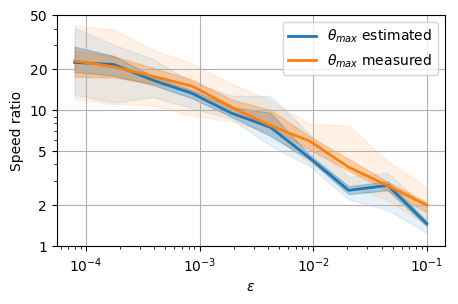
\includegraphics[scale=0.4]{images/speedratio_image}\\
				{\centering\small (a) Quadratic cost, random marginals}\label{fig:compare_a}
			\end{minipage}%
			\begin{minipage}[b]{.5\linewidth}
				\centering
				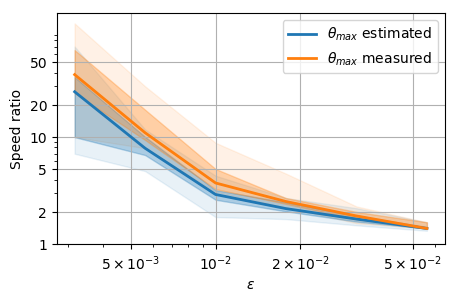
\includegraphics[scale=0.4]{images/speedratio_ML}\\
				{\centering\small (b) Random cost, uniform marginals}\label{fig:compare_b}
			\end{minipage}
		\end{tcolorbox}
	\end{minipage}
}


%----------------------------------------------------------------------------------------
%	REFERENCES
%----------------------------------------------------------------------------------------


\headerbox{References}{name=references,below=expe,column=2}{
	\small
	\begin{tabular}{r p{0.67\textwidth}}
		{[Cuturi, 2013]} & M. Cuturi. Sinkhorn distances: Lightspeed computation of optimal transport. {\it Advances in Neural Information Processing Systems 26}, 2013.\\
		{[Benamou et al., 2015]} & Benamou, J.-D., Carlier, G., Cuturi, M., Nenna, L., and Peyr\'e, G. (2015).
		{\it Iterative Bregman projections for regularized transportation problems.} SIAM Journal on Scientific
		Computing, 37(2):A1111–A1138.\\
		{[Sinkhorn, 1964]} & Sinkhorn, R. (1964). {\it A relationship between arbitrary positive matrices and doubly stochastic matrices.} The annals of mathematical statistics, 35(2):876–879.
	\end{tabular}
}


%----------------------------------------------------------------------------------------
%	Notations and definitions
%----------------------------------------------------------------------------------------

\headerbox{Sinkhorn-Knopp Algorithm}{name=Sinkhorn,column=0,below=intro,bottomaligned=references}{
	We aim at numerically solving the entropic regularization of optimal transport:
	\begin{equation} \label{eq:problem}
	\gamma^* = \argmin_{\gamma \in \Ccal_1 \cap \Ccal_2}
	\scal{c}{\gamma} + \epsilon \KL(\gamma,\One).
	\end{equation}
	In this equation, $\Ccal_1$ and $\Ccal_2$ are the marginal constraint sets corresponding to two discrete measures $\mu^1$ and $\mu^2$,
	and where $\KL$ is the Kullback--Leibler divergence.
	\begin{gather*}
	\Ccal_1 = \left\{ \gamma \mid A_1 \gamma = \mu^1 \right\},
	\quad\quad\quad
	\Ccal_2 = \left\{ \gamma \mid A_2 \gamma = \mu^2 \right\}.\\
	\KL(\gamma,\xi) = \sum_{i,j} \gamma_{i,j} \left( \log \left( \frac{\gamma_{i,j}}{\xi_{i,j}} \right) -1  \right) + \sum_{i,j} \xi_{i,j}.
	\end{gather*}
	\begin{minipage}{0.6\textwidth}
		As problem (\ref{eq:problem}) is strictly convex, it has exactly one solution, that can be written equivalently as the \emph{Bregman projection} of $\gamma^0 = e^{-c/\epsilon}$ onto a convex set:
		\begin{gather*}
		P_{\Ccal}(\xi) := \argmin_{\gamma \in \Ccal} \KL(\gamma,\xi),\\
		\text{(\ref{eq:problem})} \quad \Longleftrightarrow \quad \gamma^* = P_{\Ccal_1 \cap \Ccal_2}(\gamma^0).
		\end{gather*}
		Whereas projecting onto $\Ccal_1 \cap \Ccal_2$ is challenging, projecting onto $\Ccal_1$ or $\Ccal_2$ individually is simply performed by scaling the rows or columns of the matrix so that the corresponding marginal sum is correct.
		Operator $\oslash$ denotes element-wise division:
		\begin{align*}\label{scaling}
		P_{\Ccal_1}(\gamma) &= \diag(a) \gamma &\text{with}\quad
		a &=  {\mu^1}\oslash{A_1 \gamma} \\
		P_{\Ccal_2}(\gamma) &= \gamma \diag(b) &\text{with}\quad
		b &= {\mu^2}\oslash{A_2 \gamma}\nonumber
		\end{align*}
	\end{minipage}
	\begin{minipage}{0.39\textwidth}
		\begin{tcolorbox}[/tcb/size=small, /tcb/top=2.0mm]
			\centering
			\begin{tikzpicture}
\fill (-0.500000,4.000000) circle (2pt) node[above] (gamma0) {$\gamma^0$};
\fill (0,0) circle (2pt) node[right] {$\gamma^*$};
\draw[dashed] (-0.500000,4.000000) -- (0.000000,4.000000)
(-1.723077,3.015385) -- (0.000000,4.000000)
(-1.723077,3.015385) -- (0.000000,3.015385)
(-1.298935,2.273136) -- (0.000000,3.015385)
(-1.298935,2.273136) -- (0.000000,2.273136)
(-0.979197,1.713595) -- (0.000000,2.273136)
(-0.979197,1.713595) -- (0.000000,1.713595)
(-0.738164,1.291787) -- (0.000000,1.713595)
(-0.738164,1.291787) -- (0.000000,1.291787)
(-0.556462,0.973809) -- (0.000000,1.291787)
(-0.556462,0.973809) -- (0.000000,0.973809)
(-0.419487,0.734102) -- (0.000000,0.973809)
(-0.419487,0.734102) -- (0.000000,0.734102)
(-0.316228,0.553400) -- (0.000000,0.734102)
(-0.316228,0.553400) -- (0.000000,0.553400)
(-0.238388,0.417178) -- (0.000000,0.553400)
(-0.238388,0.417178) -- (0.000000,0.417178)
(-0.179708,0.314488) -- (0.000000,0.417178)
(-0.179708,0.314488) -- (0.000000,0.314488)
(-0.135472,0.237076) -- (0.000000,0.314488)
(-0.135472,0.237076) -- (0.000000,0.237076)
(-0.102125,0.178719) -- (0.000000,0.237076)
(-0.102125,0.178719) -- (0.000000,0.178719)
(-0.076987,0.134726) -- (0.000000,0.178719)
(-0.076987,0.134726) -- (0.000000,0.134726)
(-0.058036,0.101563) -- (0.000000,0.134726)
(-0.058036,0.101563) -- (0.000000,0.101563)
(-0.043750,0.076563) -- (0.000000,0.101563)
(-0.043750,0.076563) -- (0.000000,0.076563)
(-0.032981,0.057717) -- (0.000000,0.076563)
(-0.032981,0.057717) -- (0.000000,0.057717)
(-0.024863,0.043509) -- (0.000000,0.057717)
(-0.024863,0.043509) -- (0.000000,0.043509)
(-0.018743,0.032799) -- (0.000000,0.043509)
(-0.018743,0.032799) -- (0.000000,0.032799)
(-0.014129,0.024726) -- (0.000000,0.032799)
(-0.014129,0.024726) -- (0.000000,0.024726)
(-0.010651,0.018639) -- (0.000000,0.024726)
(-0.010651,0.018639) -- (0.000000,0.018639)
(-0.008029,0.014051) -- (0.000000,0.018639)
(-0.008029,0.014051) -- (0.000000,0.014051)
(-0.006053,0.010592) -- (0.000000,0.014051)
(-0.006053,0.010592) -- (0.000000,0.010592)
(-0.004563,0.007985) -- (0.000000,0.010592)
(-0.004563,0.007985) -- (0.000000,0.007985)
(-0.003440,0.006020) -- (0.000000,0.007985)
(-0.003440,0.006020) -- (0.000000,0.006020)
(-0.002593,0.004538) -- (0.000000,0.006020)
(-0.002593,0.004538) -- (0.000000,0.004538)
(-0.001955,0.003421) -- (0.000000,0.004538)
(-0.001955,0.003421) -- (0.000000,0.003421)
(-0.001474,0.002579) -- (0.000000,0.003421)
(-0.001474,0.002579) -- (0.000000,0.002579)
(-0.001111,0.001944) -- (0.000000,0.002579)
(-0.001111,0.001944) -- (0.000000,0.001944)
(-0.000837,0.001465) -- (0.000000,0.001944)
(-0.000837,0.001465) -- (0.000000,0.001465)
(-0.000631,0.001105) -- (0.000000,0.001465)
(-0.000631,0.001105) -- (0.000000,0.001105)
(-0.000476,0.000833) -- (0.000000,0.001105)
(-0.000476,0.000833) -- (0.000000,0.000833)
(-0.000359,0.000628) -- (0.000000,0.000833)
(-0.000359,0.000628) -- (0.000000,0.000628)
(-0.000270,0.000473) -- (0.000000,0.000628)
(-0.000270,0.000473) -- (0.000000,0.000473)
(-0.000204,0.000357) -- (0.000000,0.000473)
(-0.000204,0.000357) -- (0.000000,0.000357)
(-0.000154,0.000269) -- (0.000000,0.000357)
(-0.000154,0.000269) -- (0.000000,0.000269)
(-0.000116,0.000203) -- (0.000000,0.000269)
(-0.000116,0.000203) -- (0.000000,0.000203)
(-0.000087,0.000153) -- (0.000000,0.000203)
(-0.000087,0.000153) -- (0.000000,0.000153)
(-0.000066,0.000115) -- (0.000000,0.000153)
(-0.000066,0.000115) -- (0.000000,0.000115)
(-0.000050,0.000087) -- (0.000000,0.000115)
(-0.000050,0.000087) -- (0.000000,0.000087)
(-0.000037,0.000065) -- (0.000000,0.000087)
(-0.000037,0.000065) -- (0.000000,0.000065)
(-0.000028,0.000049) -- (0.000000,0.000065)
(-0.000028,0.000049) -- (0.000000,0.000049)
(-0.000021,0.000037) -- (0.000000,0.000049)
(-0.000021,0.000037) -- (0.000000,0.000037)
(-0.000016,0.000028) -- (0.000000,0.000037)
(-0.000016,0.000028) -- (0.000000,0.000028)
(-0.000012,0.000021) -- (0.000000,0.000028)
(-0.000012,0.000021) -- (0.000000,0.000021)
(-0.000009,0.000016) -- (0.000000,0.000021)
(-0.000009,0.000016) -- (0.000000,0.000016)
(-0.000007,0.000012) -- (0.000000,0.000016)
(-0.000007,0.000012) -- (0.000000,0.000012)
(-0.000005,0.000009) -- (0.000000,0.000012)
(-0.000005,0.000009) -- (0.000000,0.000009)
(-0.000004,0.000007) -- (0.000000,0.000009)
(-0.000004,0.000007) -- (0.000000,0.000007)
(-0.000003,0.000005) -- (0.000000,0.000007)
(-0.000003,0.000005) -- (0.000000,0.000005)
(-0.000002,0.000004) -- (0.000000,0.000005)
(-0.000002,0.000004) -- (0.000000,0.000004)
(-0.000002,0.000003) -- (0.000000,0.000004)
(-0.000002,0.000003) -- (0.000000,0.000003)
(-0.000001,0.000002) -- (0.000000,0.000003)
(-0.000001,0.000002) -- (0.000000,0.000002)
(-0.000001,0.000002) -- (0.000000,0.000002)
(-0.000001,0.000002) -- (0.000000,0.000002)
(-0.000001,0.000001) -- (0.000000,0.000002)
(-0.000001,0.000001) -- (0.000000,0.000001)
(-0.000001,0.000001) -- (0.000000,0.000001)
(-0.000001,0.000001) -- (0.000000,0.000001)
(-0.000000,0.000001) -- (0.000000,0.000001)
(-0.000000,0.000001) -- (0.000000,0.000001)
(-0.000000,0.000001) -- (0.000000,0.000001)
(-0.000000,0.000001) -- (0.000000,0.000001)
(-0.000000,0.000000) -- (0.000000,0.000001)
(-0.000000,0.000000) -- (0.000000,0.000000)
(-0.000000,0.000000) -- (0.000000,0.000000)
(-0.000000,0.000000) -- (0.000000,0.000000)
(-0.000000,0.000000) -- (0.000000,0.000000)
(-0.000000,0.000000) -- (0.000000,0.000000)
(-0.000000,0.000000) -- (0.000000,0.000000)
(-0.000000,0.000000) -- (0.000000,0.000000)
(-0.000000,0.000000) -- (0.000000,0.000000)
(-0.000000,0.000000) -- (0.000000,0.000000)
(-0.000000,0.000000) -- (0.000000,0.000000)
(-0.000000,0.000000) -- (0.000000,0.000000)
(-0.000000,0.000000) -- (0.000000,0.000000)
(-0.000000,0.000000) -- (0.000000,0.000000)
(-0.000000,0.000000) -- (0.000000,0.000000)
(-0.000000,0.000000) -- (0.000000,0.000000)
(-0.000000,0.000000) -- (0.000000,0.000000)
(-0.000000,0.000000) -- (0.000000,0.000000)
(-0.000000,0.000000) -- (0.000000,0.000000)
(-0.000000,0.000000) -- (0.000000,0.000000)
(-0.000000,0.000000) -- (0.000000,0.000000)
(-0.000000,0.000000) -- (0.000000,0.000000)
(-0.000000,0.000000) -- (0.000000,0.000000)
(-0.000000,0.000000) -- (0.000000,0.000000)
(-0.000000,0.000000) -- (0.000000,0.000000)
(-0.000000,0.000000) -- (0.000000,0.000000)
(-0.000000,0.000000) -- (0.000000,0.000000)
(-0.000000,0.000000) -- (0.000000,0.000000)
(-0.000000,0.000000) -- (0.000000,0.000000)
(-0.000000,0.000000) -- (0.000000,0.000000)
(-0.000000,0.000000) -- (0.000000,0.000000)
(-0.000000,0.000000) -- (0.000000,0.000000)
(-0.000000,0.000000) -- (0.000000,0.000000)
(-0.000000,0.000000) -- (0.000000,0.000000)
(-0.000000,0.000000) -- (0.000000,0.000000)
(-0.000000,0.000000) -- (0.000000,0.000000)
(-0.000000,0.000000) -- (0.000000,0.000000)
(-0.000000,0.000000) -- (0.000000,0.000000)
(-0.000000,0.000000) -- (0.000000,0.000000)
(-0.000000,0.000000) -- (0.000000,0.000000)
(-0.000000,0.000000) -- (0.000000,0.000000)
(-0.000000,0.000000) -- (0.000000,0.000000)
(-0.000000,0.000000) -- (0.000000,0.000000)
(-0.000000,0.000000) -- (0.000000,0.000000)
(-0.000000,0.000000) -- (0.000000,0.000000)
(-0.000000,0.000000) -- (0.000000,0.000000)
(-0.000000,0.000000) -- (0.000000,0.000000)
(-0.000000,0.000000) -- (0.000000,0.000000)
(-0.000000,0.000000) -- (0.000000,0.000000)
(-0.000000,0.000000) -- (0.000000,0.000000)
(-0.000000,0.000000) -- (0.000000,0.000000)
(-0.000000,0.000000) -- (0.000000,0.000000)
(-0.000000,0.000000) -- (0.000000,0.000000)
(-0.000000,0.000000) -- (0.000000,0.000000)
(-0.000000,0.000000) -- (0.000000,0.000000)
(-0.000000,0.000000) -- (0.000000,0.000000)
(-0.000000,0.000000) -- (0.000000,0.000000)
(-0.000000,0.000000) -- (0.000000,0.000000)
(-0.000000,0.000000) -- (0.000000,0.000000)
(-0.000000,0.000000) -- (0.000000,0.000000)
(-0.000000,0.000000) -- (0.000000,0.000000)
(-0.000000,0.000000) -- (0.000000,0.000000)
(-0.000000,0.000000) -- (0.000000,0.000000)
(-0.000000,0.000000) -- (0.000000,0.000000)
(-0.000000,0.000000) -- (0.000000,0.000000)
(-0.000000,0.000000) -- (0.000000,0.000000)
(-0.000000,0.000000) -- (0.000000,0.000000)
(-0.000000,0.000000) -- (0.000000,0.000000)
(-0.000000,0.000000) -- (0.000000,0.000000)
(-0.000000,0.000000) -- (0.000000,0.000000)
(-0.000000,0.000000) -- (0.000000,0.000000)
(-0.000000,0.000000) -- (0.000000,0.000000)
(-0.000000,0.000000) -- (0.000000,0.000000)
(-0.000000,0.000000) -- (0.000000,0.000000)
(-0.000000,0.000000) -- (0.000000,0.000000)
(-0.000000,0.000000) -- (0.000000,0.000000)
(-0.000000,0.000000) -- (0.000000,0.000000)
(-0.000000,0.000000) -- (0.000000,0.000000)
(-0.000000,0.000000) -- (0.000000,0.000000)
(-0.000000,0.000000) -- (0.000000,0.000000)
(-0.000000,0.000000) -- (0.000000,0.000000)
(-0.000000,0.000000) -- (0.000000,0.000000)
(-0.000000,0.000000) -- (0.000000,0.000000)
(-0.000000,0.000000) -- (0.000000,0.000000)
(-0.000000,0.000000) -- (0.000000,0.000000)
(-0.000000,0.000000) -- (0.000000,0.000000)
(-0.000000,0.000000) -- (0.000000,0.000000)
;
\draw (-0.000000,-0.400000) -- (0.000000,4.400000) node[right] {$\mathcal{C}_1$};
\draw (0.228571,-0.400000) -- (-2.514286,4.400000) node[right] {$\mathcal{C}_2$};
\end{tikzpicture}

			\captionof{figure}{The Sinkhorn--Knopp algorithm iterates Bregman projections on the two constraint sets.}
		\end{tcolorbox}
	\end{minipage}
	
	As shown in [Bregman, 1964], the solution can be computed by alternating Bregman projections. The main idea of the Sinkhorn--Knopp algorithm can therefore be written as:
	\begin{equation}
	\lim P_{\Ccal_2}\circ P_{\Ccal_1} \circ \ldots \circ P_{\Ccal_2} \circ P_{\Ccal_1} (\gamma^0) = \gamma^*
	\end{equation}
	This algorithm converges linearly: if we denote by $\gamma^\ell = (P_{\Ccal_2} \circ P_{\Ccal_1})^{(\ell)}(\gamma^0)$ the $\ell$-th iterate, then
	\[ \norm{\gamma^\ell - \gamma^*} = \mathcal{O}\left((1-\eta)^\ell \right) , \quad \eta > 0 \]
}

%----------------------------------------------------------------------------------------
% Main result
%----------------------------------------------------------------------------------------

\headerbox{Lyapunov Function}{name=lyapunov,column=1,below=intro,bottomaligned=Sinkhorn}{
	There is no general proof of global convergence for iterative overrelaxed Bregman projections. In order to ensure convergence, we use a Lyapunov function.
	\begin{tcolorbox}[size=small]
    	Choose $F(\gamma)$ continuous, coercive function whose unique minimizer is $\gamma^*$.\\
    	Choose $\theta_1(\gamma)$, $\theta_2(\gamma)$ continuous functions, such that
    	\begin{equation*}\label{eq:cond_theta_k}
    	\forall k \in \{1,2\}, \, \forall \gamma \notin \Ccal_k,\quad\quad
    	F(P_{\Ccal_k}^{\theta_k(\gamma)}(\gamma)) < F(\gamma).
    	\end{equation*}
    	Alternately iterate $P_{\Ccal_1}^{\theta_1}$ and $P_{\Ccal_2}^{\theta_2}$, starting from $\gamma^0 = e^{-c/\epsilon}$.\\
    	This process converges to $\gamma^*$.
    \end{tcolorbox}
    Our choice of Lyapunov function is: \[F(\gamma) := \KL(\gamma^*,\gamma)\]
    It should be noted that this function decreases for regular Bregman projections.
    
    \begin{minipage}{0.35\textwidth}
    	\begin{tcolorbox}[size=small]
    	\centering
    	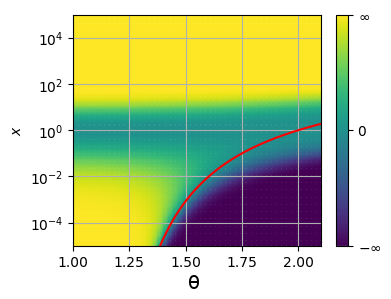
\includegraphics[width=\textwidth]{images/cvgce_zone_2.png}
    	\captionof{figure}{
    		Function $\varphi_\theta(x)$ is positive above the red line, negative below.}
    	\end{tcolorbox}
    \end{minipage}
    \begin{minipage}{0.65\textwidth}
    	The difference between two evaluations of the function can be computed directly thanks to the formula:
    	\begin{equation*} \label{eq:kl_diff_scal}
    	F(\gamma) - F(P^\theta_{\Ccal_k}(\gamma)) = 
    	\scal{\mu^k}{\varphi_\theta \left((A_k \gamma) \oslash \mu^k \right)}.
    	\end{equation*}
    	We want this difference to be positive. A sufficient condition is that every coordinate of $\varphi_\theta \left((A_k \gamma) \oslash \mu^k \right)$ be positive. Functions $\theta_1, \theta_2$ are crafted for this purpose.
    	\begin{gather*}
    	\Theta^*(u) := \max \left\{\theta \mid \varphi_\theta(u) \ge 0 \right\}
    	\\
    	\Theta(u) := clip_{[1,\theta_0]}(\Theta^*(\min u)-\delta)\\
    	k \in \{1,2\}, \quad \theta_k (\gamma) := \Theta((A_k \gamma) \oslash \mu^k)
    	\end{gather*}
    \end{minipage}
    This adaptive choice allows to choose the overrelaxation parameter $\theta_0$ that is used asymptotically. A linear study around the solution shows that overrelaxation modifies the eigenvalues in a predictable way: in particular, if the linear convergence rate of the Sinkhorn--Knopp algorithm is $1-\eta$, then the optimal asymptotic overrelaxation parameter is $\theta_0 = \frac{2}{1+\sqrt{\eta}}$.
}







\end{poster}

\end{document}